% !TeX spellcheck = en_GB
\chapter{Method and Implementation}
\section{Gene Model}
This chapter introduces a function called \mintinline{python}{gene_model}, which is an extension of the \textit{msprime} library (v. 1.3.1) \cite{msprime_github}.
The final model, documentation and examples are available on GitHub\footnote{\href{https://github.com/not-a-feature/pangenome-gene-transfer-simulation/}{github.com/not-a-feature/pangenome-gene-transfer-simulation}}
This function simulates the evolutionary process of gene gain and loss by, among other things, adapting the  \mintinline{python}{sim_mutations} function using a custom matrix mutation model.

In this adaptation, instead of simulating single nucleotide mutations, each event is either a complete gene gain or loss.
Therefore, we use a Markov model with two distinct states for each site: `absent' (0) and `present' (1) with a possible transition between them.
As \textit{msprime} works with a finite genome with $s$ sites, this approach ignores Dollo's law of irreversibility and contradicts the \ac{IMG}, stating that a lost gene cannot be regained.
To keep the probability of a gene being lost and regained low and follow the \ac{IMG}, a large genome with many sites is used.

The model uses a matrix to determine the probability of transitions between these two states, influenced by the rates of gene gain $\theta$ and gene loss $\rho$.
While gene gain is defined as a rate over the whole genome, gene loss only applies to individual sites.
It must therefore be rescaled by the total number of sites $s$.

In addition, \textit{msprime} operates with a predetermined event rate.
Therefore, the probabilities of gene gain and loss are adjusted proportionally:

\begin{equation}
    \begin{split}
        P_\theta & = \frac{\theta}{\theta + \rho \cdot s}       \\
        P_\rho   & = \frac{\rho \cdot s}{\theta + \rho \cdot s}
    \end{split}
\end{equation}


Since \textit{msprime} only traces lineages up to the \ac{MRCA}, this node needs a certain number of genes, otherwise the gene frequency spectrum will be skewed towards less frequent genes.
This can be done by using a root distribution of present genes.

Using the Poisson limit theorem, it is possible to approximate binomial distributions for large samples and small probabilities by a Poisson distribution.
This allows us to model the distribution of genes in the \ac{MRCA} node as a Poisson distribution around the expected average number of genes:
\begin{equation}
    n_\text{present} = \text{Poisson}(\frac{\theta}{\rho})
\end{equation}

The most efficient way to mark genes as `present' is to modify the sites table in \textit{tskit} directly.
By marking only the present genes and omitting the absent ones, further reduction in run time is achieved.
Since the required number of present genes is already established at the root node, an absent state should be returned whenever \textit{msprime} draws from the root distribution.

Performance analysis shows that adding all genes simultaneously using the build in \mintinline{python}{add_columns} method, focusing only on `present' genes, is significantly faster.
It outperforms the other approaches - setting both present and absent genes, or setting each position individually - by a factor of 2 to 10 in speed.

\section{Horizontal Gene Transfer}
Following the logic of the standard simulation loop, the model first calculates a random exponential waiting time weighted by the sum of segment length.
If, among all other possible events, \ac{HGT} is the one with the shortest waiting time,
the model randomly selects an existing individual (line) and a recipient segment (\mintinline{python}{y}) along that individual (Step I in \ref{fig:hgt-tree-hgt}).
Two breaks are placed at a random position within segment \mintinline{python}{y}, creating a new segment (\mintinline{python}{alpha}).
\mintinline{python}{alpha} has a length of one and represents a single gene.
This segment is now duplicated (\mintinline{python}{alpha'}) and modified so that it has no explicit origin, previous or subsequent segment associations, reflecting its status as a gene transfer line (Step II  in \ref{fig:hgt-tree-hgt}).
The donor segment is named \mintinline{python}{alpha'} or \textit{alpha prime}.
The number of segments at a given position are tracked and stored in a binary search tree (AVL tree).
By duplicating \mintinline{python}{alpha}, this number needs to be increased by one.
The key characteristic of an AVL tree is its height-balancing property: the heights of the two child subtrees of any node differ by at most one.
This ensures that the tree remains balanced, maintaining a logarithmic height relative to the number of nodes, $n$.
Consequently, operations such as lookup, insertion, and deletion can be performed in $O(\log n)$ time in both average and worst cases.
Following these adjustments, the rate maps are updated with the new lineages.
In certain edge-cases the handling of this process requires special attention.

If the alpha segment exactly matches the boundaries of the y segment\\
(i.e., \mintinline{python}{y.left == alpha.left and y.right == alpha.right}),
which can occur in horizontal gene transfer or gene conversion lineages, there is no need to insert breaks or change the recipient segment.

Furthermore, if the selected recipient segment is the first segment in the chain and its left breakpoint is equal to the left boundary of the recipient segment, then alpha must replace the recipient as the head of the lineage.
Otherwise, an inconsistent segment chain would be created.

A new node (\mintinline{python}{HM}) of the newly created class \mintinline{python}{HORIZONTAL_MERGE} is added to act as the new parent of the original segments.
Since a free-floating segment (\mintinline{python}{alpha'}) is not possible, it is linked to another new node (\mintinline{python}{HG}) of class \mintinline{python}{HORIZONTAL_GENE} (Step II),
which has a direct parent (\mintinline{python}{HP}) of class \mintinline{python}{HORIZONTAL_PARENT}.
This newly formed ancestor is then treated in the same way as any other line within the model, including possible future mergers with other lines.
\newpage
In order to represent the gene transfer event, and to be able to place mutations, edges are introduced (Step III  in \ref{fig:hgt-tree-hgt}).
These edges span from:
\begin{itemize}
    \item \mintinline{python}{HM} to \mintinline{python}{RN} over the whole line (segment chain).
    \item \mintinline{python}{HP} to \mintinline{python}{HM} over the \mintinline{python}{alpha} region.
    \item \mintinline{python}{HP} to \mintinline{python}{HG} over the \mintinline{python}{alpha} region.
\end{itemize}
Due to the strict structural integrity checks of \textit{tskit}, the \mintinline{python}{HP-HM} edge is appended to a separate edge buffer and are merged in the latter described mutation placing algorithm.

\begin{figure}[]
    \centering
    \includegraphics[width=0.49\textwidth]{figures/hgt.pdf}
    \includegraphics[width=0.49\textwidth]{figures/tree_with_hgt.pdf}
    \caption[Logic of HGT events.]{Schematics of a single HGT event divided into 3 steps (from top to bottom) (left) and in the context of a complete tree (right).}
    \label{fig:hgt-tree-hgt}
\end{figure}

Given the potential for new \ac{HGT} lineages to emerge at a faster rate than the occurrence of common ancestor events, there is a risk of divergence in the simulation.
To mitigate this, we set the \ac{HGT} rate to zero once the elapsed (simulated) time exceeds five times the time expected in the absence of \ac{HGT} events.
This ensures that no new \ac{HGT} lineages are generated.
The time to the next coalescent event is modelled using an exponential distribution with parameter $\lambda = n(n-1)$,
where the $n$ corresponds to the current number of lineages at the given time step  (see \ref{subsec:kingman}).
\newpage
Given that the expected value of an exponential distribution, and thus the time to the next coalescent event, is $1/\lambda$,
the expected time for all lineages to coalesce - assuming no \ac{HGT}, gene conversion, or other lineage-modifying events - is denoted as,
$\mathbb{E}_\text{time}$ and calculated as follows:
\begin{equation}
    \begin{split}
        \mathbb{E}_\text{time} & = \sum_{i=2}^{i=n} \frac{1}{i(i-1)}                                                                                                         \\
        & = \sum_{i=2}^{i=n} \frac{1}{i-1} - \frac{1}{i}                                                                                              \\
        & = \left( \frac{1}{1} - \frac{1}{2} \right) + \left( \frac{1}{2} - \frac{1}{3} \right) + \cdots + \left( \frac{1}{n-1} - \frac{1}{n} \right) \\
        & \text{In a telescoping series, intermediate terms cancel out,}                                                                              \\
        & \text{leaving only the first term of the first and last term oft the last fraction.}                                                        \\
        & = 1 - \frac{1}{n}
    \end{split}
\end{equation}
We therefore use $5\times\mathbb{E}_\text{time} = 5 - \frac{5}{n}$ is as limit.

\section{Mutation Simulation}

An adaptation of the regular \mintinline{python}{sim_mutation} function from \textit{msprime} is necessary as the horizontal gene transfer tree structures
cannot be represented as a \mintinline{python}{tskit.TreeSequence} in the current version of \textit{tskit}.
This restriction is due to \textit{tskit's} rule that each node may have only one parent per position, as described in the previous section.
Furthermore, the mutation algorithm lacks the ability to detect mutations occurring on \ac{HGT} edges and their interactions with regular mutations.

The structure of the adapted mutation simulation is based on the original implementation and proceeds as follows:

\begin{enumerate}
    \item \textbf{Placement of mutations}: In this step, mutations are assigned to each edge.
          The number of mutations is drawn from a Poisson distribution with a mean based on their length, which represents the time between parent and child, and span, which is the distance from left to right boundaries.
          This step randomly determines the location within these boundaries for a mutation to occur, noting only the presence of a mutation without specifying its type or any other information.
          \newpage
    \item \textbf{Tree traversal}:  For each position in the genome, this process records the corresponding tree structure.
          It traces the edges from the root node responsible for that position (\mintinline{python}{edge.left <= bp_l and bp_r <= edge.right}) to a leaf, documenting any parent-child relationships along the way.
          Since the genome is divided into segments, and the tree is identical for each position in that segment, it is sufficient to compute this tree structure for each segment, which improves efficiency.
    \item \textbf{Apply mutations}: The first mutation, which is the oldest in time, is applied based on the mutation model.
          For the subsequent mutation, the tree, which was recorded in the previous step, is traversed upwards to identify the parent mutation.
          This mutation could be on a different edge.
          For each edge the last mutation is stored in a hashmap for quick access.
          In the case of two or more parental mutations, due to multiple incoming edges (some of which are \ac{HGT} edges), a check is made to see if one represents a gene gain.
          If so, this mutation is propagated and used as the current parental state.
          The other mutation is discarded.
          A flag is stored as metadata to mark the mutation if it was affected by a \ac{HGT} event.
          To save memory, this metadata is stored as unsigned 8-bit integer, using the second least significant bit as \ac{HGT} flag.
          After determining the derived state, the hashmap is updated with the current mutation and the next one is processed.

    \item \textbf{Sentinel Mutations}: To ensure that the final state of each position is correctly calculated and, that \ac{HGT} edges are not ignored, sentinel mutations are inserted at time 0.
          These sentinel mutations are silent, i.e.
          do not change the state, but ensure that downstream algorithms, such as the genotype matrix and the GFS calculation, work correctly, as they only take the last mutation into account.
          These mutations are marked by the least significant bit of the metadata flag.

    \item \textbf{Fill the tables and remove the HGT edges}: This final step involves filling the mutation table and removing the \ac{HGT} edges to produce a valid \mintinline{python}{tskit.TreeSequence}.
\end{enumerate}

The resulting tree, now validated and embedded with mutations, is returned.
\newpage
\section{Events on a fixed tree}
To test the effects of horizontal gene transfer or gene conversion and estimate the parameters using real-world data, the simulation must follow a specified tree structure.
This feature is introduced in this chapter.
The objective is to maintain the provided tree structure while allowing regular simulation events, such as gene conversion, to occur.
The structure can be specified either by a Newick string or derived from a \mintinline{python}{tskit.TreeSequence} object.

Several structural changes were required to incorporate this functionality:
\begin{itemize}
    \item \textbf{Segment class}: The  \mintinline{python}{Segment} class is extended by a new attribute called \mintinline{python}{origin}.
          This attribute will be a set that keeps track of the lineage IDs from which the current segment originates.
          Initially, this set contains only the ID of the leaf from which the segment originated.
          During coalescence events, the origin sets of the merging segments are combined.
    \item \textbf{Newick parser}: A new parser component has been implemented to process the user-provided Newick string.
          This parser generates a list of tuples, where each tuple represents a coalescence event consisting of three elements:
          \begin{itemize}
              \item The time at which the coalescence event occurs (float).
              \item A set containing the IDs of the first lineage involved in the coalescence.
              \item A set containing the IDs of the second lineage involved in the coalescence.
          \end{itemize}
          This is archived by recursively splitting the Newick string into a left and right part until a leaf is reached.
    \item \textbf{TreeSequence parser}: Similar to the Newick parser, the \mintinline{python}{TreeSequence} parser generates a list of tuples by iterating through the edges.
          Whenever two edges point to the same parent, the time of the parent node is recorded with the IDs of the children.

\end{itemize}

The \mintinline{python}{hudson_simulate} method is adapted to handle fixed coalescence events specified in the tree.
If the current simulation time (\mintinline{python}{self.t}) has exceeded the time of the next fixed coalescence event
stored in the \mintinline{python}{coalescent_events} list (\mintinline{python}{self.coalescent_events[0][0]}),
the algorithm will deviate from its regular behaviour.
The simulation time is reset to the exact time of the coalescent event, possibly with a small epsilon value to
avoid storing two events at the same time step.
The method will first use the \mintinline{python}{get_emerged_from_lineage} method to retrieve all lineages that have emerged from the two ancestral lineages specified in the event.
Then, for each pair of lineages (one from lineage A and one from lineage B), one lineage is randomly selected to coalesce,
ensuring that the predefined tree structure is followed.
For regular coalescence events (not specified in the provided tree), the method continues its usual behaviour, randomly selecting two lines to merge or skipping the event if the lines are needed later.
As this feature can be directly incorporated into \textit{msprime} a pull request was opened\footnote{\href{https://github.com/tskit-dev/msprime/pull/2276}{https://github.com/tskit-dev/msprime/pull/2276}}.

\section{Neutrality Test and $\chi^2$ like statistic}
In order to determine whether the observed Gene Frequency Spectrum results from a process of neutral evolution with similar gene gain / gene loss parameters or is influenced by gene conversion or \ac{HGT}, we developed a statistical test.
This test, which can be divided into a direct approach and a $\chi^2$-like approach, uses both a \ac{KS} test and \ac{KDE} to evaluate \ac{GFS} patterns derived from simulating a neutral evolutionary model.
KDE is mainly used to smooth initial distributions and improve results, especially when working with small numbers of simulations.

\subsection{Direct Class Approach}
In the direct method, we match each observed gene frequency class, $g_i^n$, with its corresponding simulated distribution under neutral evolution.
These simulations are generated using the most likely parameters of a pure clonal model with gene gains and losses or the parameters of interest.
A robust reference distribution is measured by simulating 1000 times.
\begin{figure}[h]
    \centering
    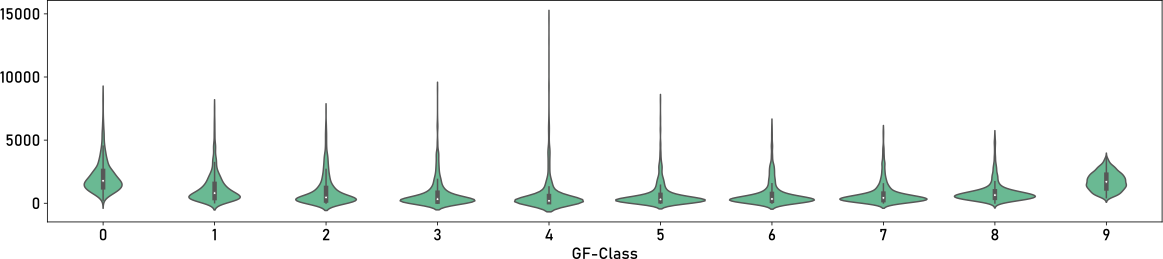
\includegraphics[width=\textwidth]{figures/gfs.pdf}
    \caption[Typical Gene Frequency Spectrum.]{Typical distribution of gene frequency classes. 10 Individuals simulated with $\theta = 1000$ and $\rho = 0.2$.}
    \label{fig:typical-gfs}
\end{figure}

The figure \ref{fig:typical-gfs} shows a typical distribution of gene frequency classes.
In this example, 10 individuals were simulated with a gene gain / gene loss rate of 1000 and 0.2 respectively.
The Kolmogorov-Smirnov test quantifies the difference between the simulated distribution and the observed value.
This is repeated for each gene frequency class.

Similar to the \ac{KS} approach, the \ac{KDE}-based direct approach fits a kernel density estimate with a Gaussian kernel to each distribution.
This results in a smooth approximation of the probability density function.
To evaluate how extreme the observed data point under the neutral evolution model is, we calculate a p-value by integrating the \ac{KDE} from the observed data point to either positive or negative infinity.
The integral represents the probability of observing a data point that is as extreme or more extreme than the observed value under neutrality.

In both the \ac{KS} test and the \ac{KDE} integration, the null hypothesis is that the two observed samples are drawn from the given distribution.
The two-tailed alternative hypothesis states that the distributions is different.

Importantly, the p-values derived from each gene frequency class are not independent.
This means that it is not possible to simply multiply them to determine the overall significance.
One solution is to use the smallest p-value, which is no longer a valid p-value in the traditional sense.
It is more likely to be smaller than the significance level, even if the null hypothesis is true for all tests.
This increased likelihood of Type I error is mitigated by directly implementing a Bonferroni correction:
\begin{equation}
    p_{\text{direct}} = \text{min}(p_{g^n_1}, ~ p_{g^n_2}, ~ ..., ~ p_{g^n_n}) \cdot n
\end{equation}

If this minimum p-value falls below our chosen significance threshold, we reject the null hypothesis of neutral evolution.
This rejection suggests that the observed \ac{GFS} could be influenced by factors other than neutral evolutionary processes, such as \ac{HGT}.

\subsection{Through a $\chi^2$-like Summary Statistic}\label{subsec:chi}
Through a $\chi^2$ -like summary statistics, we can directly measure the distance between the measured gene frequency spectrum $(g_1^n, ..., g_n^n)$, and its expected values under neutral evolution.
We define:

\begin{equation}
    \chi^2(g_1^n, ..., g_n^n) = \Sigma^n_{i=1} \frac{(g_i^n-\mathbb{E}[G_i^n])^2}{\mathbb{E}[G_i^n]}
\end{equation}
Following a similar approach, we generate many gene frequency spectra under a neutral evolutionary model.
We then compute a $\chi^2$-like statistics for each spectrum.
Unlike previous methods, this approach produces a single distribution allowing us to directly apply a \ac{KS}-test and fit a kernel density estimate.
As the $\chi^2$ value increases as the error from the expected values increases, only a one-tailed test is used.

The kernel density estimate shown in figure \ref{fig:pdf-cdf} characterises the \ac{PDF} of the $\chi^2$ values.
Together with the \ac{CDF}, a logarithmic transformation of it shows similarity to a normal distribution, although its shape is slightly skewed, indicating that the $\chi^2$ values follow a log-normal distribution.

\begin{figure}[]
    \centering
    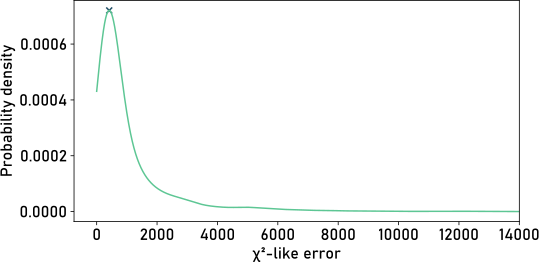
\includegraphics[height=3.5cm]{figures/pdf.pdf}
    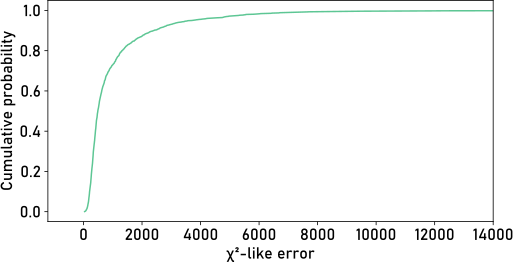
\includegraphics[height=3.5cm]{figures/cdf.pdf}
    \caption[Typical PDF and CDF.]{Typical Probability Density Function (left) and Cumulative Distribution Function (right) of $\chi^2$ values.}
    \label{fig:pdf-cdf}
\end{figure}
\newpage
To account for the variability observed between gene frequency classes, which is particularly pronounced at the boundaries ($g_1^n$ and $g_n^n$) compared to the centre, we introduce a weighting parameter to control the influence of each class.
This weight vector assigns relative importance to each gene frequency class.
By default, in the unweighted scenario, the weight vector is defined as $(w_0, w_1, \ldots, w_n)$, where each $w_i = 1$.
As these are relative weights, they must satisfy the condition $\sum_{i=0}^n w_i = n$.
The adapted $\chi^2$ -like summary statistic is now as follows:

\begin{equation}
    \chi^2(g_1^n, ..., g_n^n) = \Sigma^n_{i=1} \frac{(g_i^n-\mathbb{E}[G_i^n])^2}{\mathbb{E}[G_i^n]} w_i
\end{equation}

\section{Minimal Site Count}

While investigating the effect of the number of sites on the simulation runtime,
it became clear that a low number of sites is desirable in order to run multiple simulations efficiently and to obtain reliable neutrality test results.
However, in the infinite gene model, a high number of sites, ideally approaching infinity, is necessary as otherwise a gene gain event is likely to occur at a site where a gene already exists.
This includes gene gain events where the root ancestral state is `present'.
It is therefore desirable to find the minimum number of sites that will not significantly bias the resulting statistics.
An analytical and a computational approach have been used to do this.
For a single event the probability that a given event is a gene-gain is:
$$P_\theta = \frac{\theta}{\theta + \rho \cdot s}$$
with $s$ the total number of sites.
With that, the probability that at least one the $s$ sites is hit twice is:

\begin{equation}
    P_{\text{double}} = 1-(1-P_\theta^2)^s =  1-(1-(\frac{\theta}{\theta + \rho \cdot s})^2)^s
\end{equation}

\begin{figure}[h]
    \centering
    \includegraphics[width=0.6\textwidth]{figures/double_proba.pdf}
    \caption[Probability of double gene gain events.]{Probability that at least one double gene gain event is happening.}
    \label{fig:double-proba}
\end{figure}

The figure \ref{fig:double-proba} showed that double gene gain events remain likely, even for small gain/loss ratios, unless a very high number of sites ($>> 10^6$) is used.
The second approach looked at the effect on the $\chi^2$-like statistics.
Simulations were run with different number of sites ranging from $1000$ to $500000$.
Each simulation ($n = 10, \theta = 100, \rho = 0.1$) was repeated 1000 times.
For these simulations, the \ac{GFS} was recorded and the $\chi^2$-like statistic calculated and log-transformed.
The results were compared with a reference distribution assuming a site count of $10^6$, as the number of observed double mutations were low ($< 10$).
For a low number of sites ($s < 20000$), a t-test indicated significant deviations from the expected neutral model, as indicated by the very low p-values.
For higher $s$, the p-values increased and exceeded the $0.05$ threshold, indicating less deviation from the expected neutrality.
The table with all p-values can be found in appendix \ref{app:double-p-value}.
We therefore concluded that double gene gain can significantly bias the $\chi^2$-like statistical summary.


Despite these observations, a hard limit on the number of sites has not been implemented in order to maintain flexibility for the user.
Nevertheless, the number of double gain events is tracked to ensure the reliability of the results.
A warning is given if the frequency of these events exceeds 1\% of the total number of mutation events.

\subsection{Relocation of mutations}
Apart from as increasing the total number of sites, an alternative strategy is to relocate the double gene gain mutations.
In the case of recombination or gene conversion, different trees describe different segments of the genome.
Therefore, moving a mutation to an unused position could place it on a different tree and change its properties.
This is because mutations are more likely to occur twice in the same place on longer trees.
Consequently, the new position must be selected with the same bias, making random repositioning impractical.
Although this could be assessed by repositioning the mutation only within the bounds, this would drastically limit the number of mutations that could be repositioned.
Therefore, our implementation of random repositioning focuses only on scenarios without recombination or gene conversion.
This process involves extracting the tabular representation of the tree and creating a mask for double gene gain mutations based on the derived and parental states.
These identified mutations are then duplicated and mapped to a new, unused position and site.
To optimise computational efficiency, we access the data directly and create an array of all mutations / sites,
bypassing the resource-intensive creation of \mintinline{python}{MutationTableRow} and \mintinline{python}{SiteTableRow} objects.
While this is a fast and intuitive approach, it is limited by the number of possible new positions.
Thus, a \mintinline{python}{RuntimeError} is raised if the number of double mutations exceeds the number of free sites.

\newpage
\subsection{Genome Splitting}
An alternative approach to dealing with double gene gain events is to simulate with twice the number of sites.
This will double the number of mutations and approximately double the simulation time.
Following the simulation, we divide the mutations into a `left' and a `right' partition, ensuring an equal number of sites in each.
In the left partition, we eliminate all double gain mutations (i.e., gain mutations with gain mutations or `present' ancestral states as their parents).
On the right, we remove mutations that are not double gain mutations.
In addition, we reset the ancestral state drawn from the root distribution to `absent' to avoid sites marked as `present' without mutations.

Finally, we use the \mintinline{python}{tables.compute_mutation_parents()} function to correct any missing parental
relationships to ensure the integrity of the tree structure.
This allows us to reconstruct the tree without double mutations and similar features.

\begin{figure}[h]
    \centering
    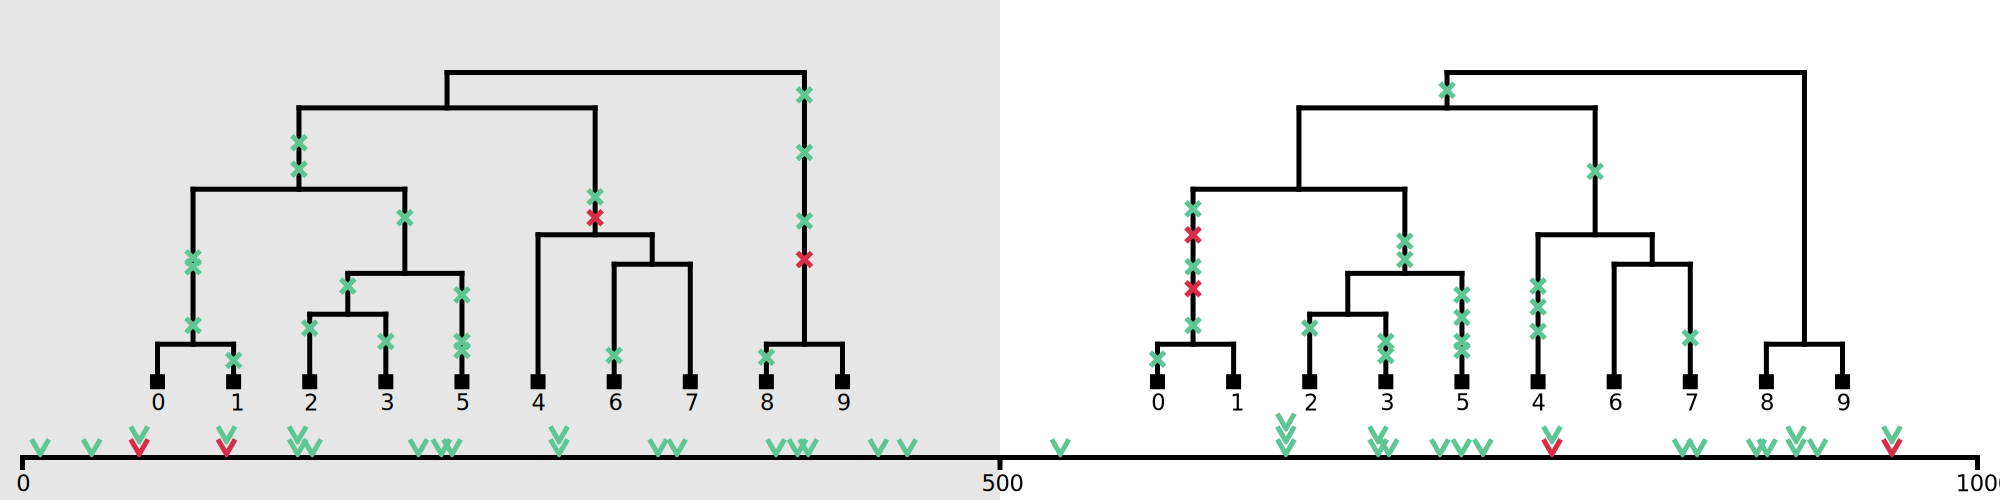
\includegraphics[width=\textwidth]{figures/tree_split_pre.pdf}\\
    \includegraphics[width=\textwidth]{figures/tree_split_post.pdf}
    \caption[Tree splitting for mutation relocation.]{Tree with mutations before (top) and after (bottom) splitting and removal of mutations.}
    \label{fig:tree-split}
\end{figure}

If, as in this example, a genome with 500 sites were desired, a simulation with 1000 sites would be used.
Here 42 mutations were simulated, 4 of which were double mutations.
On the left partition of the genome, all (2) double mutations were removed, while on the right partition only the double mutations (red) were kept.
While the genome has 1000 sites, it has the same number of present genes as a simulation with 500 under the \ac{IMG} model.

\section{Integration}
The gene gain and loss mutation model has been integrated with the customised \ac{HGT} ancestry and mutation simulation model to form a complete framework.
To provide a user-friendly interface, mutation relocation and tree fixation have also been added to this function.
Care had to be taken when relocating mutations as some sentinel mutations would be identified as double gene gain mutations.
An additional mask using the mutations' metadata has been introduced to account for this.
Due to its superior performance, the C implementation is used over the Python version whenever possible, especially when $\gamma = 0$ zero or when no \ac{HGT} events have been simulated.

\begin{table}[H]
    \label{tab:parameters}
    \begin{adjustbox}{width=\textwidth}
        \begin{tabular}{r|lll}
                     & Parameter                                      & Type                                     & Description                                                                                \\
            \hline
            $\theta$ & \mintinline{python}{theta}                     & \mintinline{python}{int}                 & Gene gain rate.                                                                            \\
            $\rho$   & \mintinline{python}{rho}                       & \mintinline{python}{float}               & Gene loss rate.                                                                            \\
                     & \mintinline{python}{ts}                        & \mintinline{python}{tskit.TreeSequence}  & \mintinline{python}{TreeSequence} to simulate gene gain and loss directly on this tree.    \\
                     & \mintinline{python}{hgt_edges}                 & \mintinline{python}{List[tskit.Edge]}    & List of HGT edges that can't be represented in the \mintinline{python}{TreeSequence}.      \\
            $n$      & \mintinline{python}{num_samples}               & \mintinline{python}{int}                 & Number of samples.                                                                         \\
            $s$      & \mintinline{python}{num_sites}                 & \mintinline{python}{int}                 & Number of sites in the genome.                                                             \\
            $\kappa$ & \mintinline{python}{gene_conversion_rate}      & \mintinline{python}{float}               & Gene conversion rate.                                                                      \\
                     & \mintinline{python}{recombination_rate}        & \mintinline{python}{int}                 & Recombination rate.                                                                        \\
            $\rho$   & \mintinline{python}{hgt_rate}                  & \mintinline{python}{float}               & Horizontal Gene Transfer rate.                                                             \\
                     & \mintinline{python}{ce_from_nwk}               & \mintinline{python}{str}                 & Tree structure in Newick format to follow during simulation.                               \\
                     & \mintinline{python}{ce_from_ts}                & \mintinline{python}{tskit.TreeSequence } & Tree structure in \mintinline{python}{TreeSequence} format to follow during simulation.    \\
                     & \mintinline{python}{check_double_gene_gain}    & \mintinline{python}{bool}                & Warning if more than 1\% of all events are double gene gain events.                        \\
                     & \mintinline{python}{double_site_relocation}    & \mintinline{python}{bool}                & Simulates with $2 \times $ \mintinline{python}{num_sites} and fixes double gain mutations. \\
                     & \mintinline{python}{relocate_double_gene_gain} & \mintinline{python}{bool}                & Repositions double gene gain mutations.                                                    \\
        \end{tabular}
    \end{adjustbox}
    \caption{Parameters of the \mintinline{python}{gene_model} function that combines the HGT ancestry simulation with the gene gain / loss model.}
\end{table}

\section{Estimating parameters for real world pangenomes}
To test the models' capabilities, we used real-world pangenomes, calculated the \ac{GFS} and optimised the simulation parameters using a \textit{Simplicial Homology Global Optimisation} and \textit{Differential Evolution} approach to match the simulated \ac{GFS} with the real ones.
Samples of multiple bacterial species we downloaded and processed by Hannah G\"otsch using \textit{PanX}.

\textit{PanX} is a software tool designed to streamline the construction and analysis of pan-genomes \cite{Ding_2017}.
It begins by using the \textit{DIAMOND} alignment algorithm to perform an all-against-all similarity search, identifying pairs of genes across the input genomes that have significant sequence similarity \cite{Buchfink_2014}.
These similarity results are then clustered using a Markov clustering algorithm, which groups genes that are likely to have a common evolutionary origin (orthologs).
As \textit{DIAMOND} focuses on proteins, \textit{PanX} has a separate process to identify and cluster non-coding genes such as ribosomal RNAs (rRNAs) using BLASTn.
To cope with the potential computational burden of analysing thousands of genomes, \textit{PanX} avoids direct all-against-all comparisons.
Instead, it clusters smaller subsets of genomes, then represents these clusters by `pseudo-genomes' and repeats this process hierarchically.
This strategy helps to maintain a near-linear growth in computational cost as the number of genomes increases.

\textit{PanX} constructs phylogenetic trees for each gene cluster using tools such as MAFFT (for alignment) and FastTree (for tree-building) \cite{Katoh_2002} \cite{Price_2010}.
These trees are carefully analysed to split gene clusters that may contain paralogs (genes related by duplication within a genome).
\textit{PanX} uses a combination of branch length thresholds and a `paralogy score' to finely separate orthologs into distinct groups.
It also has a process to address genes that may have been missed in the initial clustering, combining them based on sequence length and phylogenetic analysis.

Using alignments of core genes (present in all strains), \textit{PanX} builds a `core genome' phylogenetic tree using \textit{FastTree} and refines it using \textit{RaxML}.
This tree shows the overall evolutionary relationships between the strains.
Later, this tree is used to remove potential oversampling using \textit{PhyloThin}.

The thinned core genome trees and gene presence/absence matrices were exported and used for subsequent parameter estimation using the Simplicial Homology Global Optimisation algorithm.

The \ac{SHGO} algorithm is a method for efficiently identifying local minima in objective functions, especially when, as in our case, the function is costly to evaluate \cite{Endres_2018}.
For this we use the implementation of the \textit{SciPy} package \cite{scipy}.
As objective function we used the $\chi^2$ error of the mean \ac{GFS} of 24 simulations against the true \ac{GFS}.
This choice was a compromise between run time and variability of the error.
The algorithm uses concepts of simplicial integral homology and combinatorial topology to navigate complex problem landscapes,
which makes it useful for high-dimensional and complex applications such as exploring energy landscapes or, in our case, the $\chi^2$-like error for different parameters.
Of course this step assumes that the phylogenetic tree, computed by \textit{PanX} is correct.

\ac{SHGO} works by starting with the construction of a simplicial complex from the feasible search space.
This complex forms a topological abstraction where the vertices represent potential solutions and the simplicial links illustrate possible optimisation paths.
By approximating the homology groups of this complex, \ac{SHGO} is able to map the structure of the search space and pinpoint areas likely to contain local minima.
The search space is defined by bounds that we set to:

\begin{table}[h]
    \begin{adjustbox}{width=\textwidth}
        \begin{tabular}{llll}
            Parameter & start  & stop                               & Description                    \\
            \hline
            $\theta$  & 0.1    & average number of genes $\times 3$ & Gene gain rate.                \\
            $\rho$    & 0.0001 & number of samples                  & Gene loss rate.                \\
            $\kappa$  & 0      & 0.01                               & Gene conversion rate.          \\
            $\gamma$  & 0      & 0.01                               & Horizontal Gene Transfer rate. \\
            recomb    & 0      & 0.01                               & Recombination rate.
        \end{tabular}
    \end{adjustbox}
    \caption{Parameter search-space.}
\end{table}

based on our previous experience and runtime feasibility.

The algorithm uses intelligent sampling methods based on the vertices of the simplicial complex, guided by Sperner's lemma.
This lemma helps to approximate locally convex subdomains that are likely locations of local minima, significantly reducing the number of function evaluations required.

The other optimisation technique we used is the \ac{DE} approach by Storn and Price \cite{Diff_Evo_Storn_1997} which finds an optimal solution by evolving a population of candidate solutions over time.
Differential Evolution involves four main steps: initialization, mutation, crossover, and selection.
Initially, a population of $15$ candidate solutions is randomly generated, within our search space. We use the same bounds as in the \ac{SHGO} approach.
Each candidate solution, also called an individual, is represented as a vector.
Once the initial population is established, the algorithm proceeds to the mutation step.
In this phase, for each candidate solution in the current population, a mutant vector is generated.
This is done by selecting three distinct individuals from the population and combining them by adding the weighted difference between two of these individuals to the third one.
The mutation is followed by the crossover step which aims to increase the diversity of the population by randomly combining components of the mutant vector with the candidate vector to create a trial vector.

Finally, in the selection step, the trial vector is compared to the target vector based on their fitness values, which are determined by the objective function being minimised.
If the trial vector has a better fitness value than the candidate vector, it replaces it in the population.
This ensures that the population evolves towards better solutions over successive generations.

Once the minimisation process had converged, the parameters were recorded and further refined using a \ac{DS} approach.
This additional step is necessary as both \ac{SHGO} and \ac{DE} algorithms excel at exploring the wider $\chi^2$ value landscape,
but struggle in the final, local optimisation.

For this step, the number of simulations per evaluation of the objective function was increased
from 24 to 48 in order to reduce the variability of the $\chi^2$ like value.
The result of this process is a list representing several gene frequency spectra,
providing a distribution and $\chi^2$ like measurement indicating the fit of the simulated parameters to the true parameters.
